%!TEX root = ../template.tex
%%%%%%%%%%%%%%%%%%%%%%%%%%%%%%%%%%%%%%%%%%%%%%%%%%%%%%%%%%%%%%%%%%%
%% experiments_results.tex
%% NOVA thesis document file
%%
%% Chapter with Introduction
%%%%%%%%%%%%%%%%%%%%%%%%%%%%%%%%%%%%%%%%%%%%%%%%%%%%%%%%%%%%%%%%%%%

%%%%%%%%% TODO FUTURE WORK CHAPTER. MENCIONADO %%%%%%%%%%%%

\typeout{NT FILE experiments_results.tex}

\chapter{Experiments and Results}
\label{cha:Experiments and Results}


\section{Introduction}
\label{sub:if_you_use_this_template} 
The experiments that were built during this work, as mentioned before, started by having a more generic and simple approach, in terms of the scopes of the datasets and in terms of the dataset pre-processing steps. While we were studying the experimental results by using the evaluation metrics mentioned in the previous Methodology section, we learned more about the problems and considering the clients, CGI experts feedback and our literature, we improved our experiment to its final form.

In this section we will present the final form of the experiment that is going to be implemented as a base for the failure prediction tool. We will present all the dataset pre-processing procedures that were implemented in .NET, using Visual Studio, to acquire all the data from the CGI RMS database and to execute some of the pre-processing procedures needed in order to build the dataset. This dataset is then provided to the experiment build inside the Azure Machine Learning Studio, that is the main tool that receive the dataset and build the machine learning models that are then evaluated.

\section{Experiment}
In the presentation of our experiment, we will separate it into two steps, according to the technologies that were used. Firstly we will introduce the construction of our dataset, that contains some data pre-processing and feature engineering methods, which results in the dataset that is then provided to the next step, in the Azure Machine Learning Studio experiment.

\subsection{Dataset Acquisition and Build Up}
This first step was build in .NET, using Visual Studio, and with SQL Server, the database system where the CGI RMS data is stored.

In this first experimental phase, we are not going to refer all the study work of the signals that should be associated with a fault in a wind turbine is done, presented previously in the Methodology section.

Our dataset acquisition parameters, will have a start time, defined as the March 6th 2021, and an end date, the December 31st 2021 at 23:59:59. The sliding time windows that are going to be studied are 12 hours, 24 hours and 72 hours.
For each wind turbine fault, we will generate a dataset according to different sliding time windows.

%NOTA: FOI DESCOBERTO UM ERRO NO PROCESSO DE AQUISICAO PARA A CONSTRUCAO DAS RUNNING SUMMARIES
%ESTA FIXO EM 6H. PARA JÁ, VOU ESCREVER EM BAIXO O VALOR CORRETO, MAS VOU ANALISAR A POSSIBILIDADE DE ESCONDER ESTE RESULTADO

%METER UMA TABELA DE RESUMO DOS PARAMETEROS

\begin{enumerate}
    \item 
Firstly we acquire the data from the signals that have good quality. For each feature, it is generated the running summaries, mentioned earlier in the Methodology section, with the generation of these features considering the average, standard deviation, minimum and maximum of each signal for the last 6 hours.
The parameter number of hours defined in this step was fixed since this technique was applied later in this master thesis work and from the knowledge of the CGI experts, we consider that looking 6 hours before it is good to compare mainly abrupt changes in a wind turbine behavior.
It is mentioned in the Future Work section, an improvement that we consider that should be studied after this master thesis work.

    \item
After the acquisition of the signals data, with the running summaries features, it is removed from the features column, all the features that have more than 50\% of null rows. We have to do this step, since if we keep these features, we will have to remove the null rows and that will lead to a big amount of timestamps being removed only because of one signal.
Then, after the analysis of the invalid features is concluded, the remaining null rows are removed.

    \item
Then we step up to the failure events data acquisition, that it is generated according to the current sliding time window. In this step, besides the acquisition of the timestamps that have a failure event, it is also generated the fault column, mentioned earlier in the Methodology section.

    \item
After the acquisition of the timestamps that correspond to a failure event and the construction of the fault column, it is built an auxiliar column, the fault category.

    \item
Our final step, is a simple merge of the signals data and the faults data, so that we have only the corresponding timestamps that exist in both tables obtained earlier. To finalize the dataset, it is done a last check to delete rows with null features, whetever they exist.

\end{enumerate}

%METER PRINT DA EXPERIENCIA DOS STEPS DO CODIGO COM NRS ASSOCIADOS A CADA STEP

After this process of the dataset generation, we have generated all datasets for each fault and wind turbine, one .csv file per sliding time window, meaning that for each wind turbine fault we have 3 .csv files, one for the sliding time window of 12h, one for the 24h and another for the 72h.

%METER AQUI UM DIAGRAMA DE PROCESSO A REPRESENTAR
%DIAGRAMA DE PROCESSO A REPRESENTAR ESTE PROCESSO (TODO)

\subsection{Azure Machine Learning Studio Experiment}
Having the datasets available to provide to our Azure Machine Learning Studio Experiment, we can start running our final experiment.
In this subsection, we will introduce each module that is going to run in our experiment, providing a brief explanation on what each module is going to do and justifying our decisions according to what was introduced earlier in the methodology section. In Figure 6.1 it is briefly represented in a diagram the complete experiment that is going to be explained later in this section.
Our experiment is divided into three parts that are equal to each other. In each part, we will provide a different dataset for each fault with each file (.csv) varying by the time window of that dataset, as presented before.

\begin{enumerate}
    \item{Import Data:}
Component that imports data. In our case, we will import data from the Azure Storage that contains all the .csv files with the dataset. The data that comes from the .csv file contains all the available data for that particular fault and time window, this means since March 2021 to the end of December 2021.

    \item{Separate the Training Dataset from the Final Evaluation Dataset:}
Using the 'Apply SQL Transformation' module, we will split our import data into the first split dataset, that we call Training Dataset and that will contain the data from March 2021 to the end of September 2021, and the second split dataset, that we call Final Evaluation Dataset and that will contain the data from October 2021 to the end of December 2021.

The next steps uses the first split dataset, the Training dataset. The second split dataset, called Final Evaluation Dataset, is used in the steps presented at the end of this subsection.
    
    \item{Edit Metadata:}
This component allows us to set to each column some metadata info that is useful to improve the performance of the models.
    
    \item{Filter Based Feature Selection:}
This component goal is to identify and select the "columns in the input dataset that have the greatest predict power" \cite{AZURE_MACHINE_LEARNING}. This module provide the option to choose the correlation method to classify the prediction power of each feature. The available methods are Pearson correlation and Chi-squared values.

We selected Chi-squared for the correlation method since it is refereed in \cite{OLD_41_WIND} and \cite{MLMistery_Feature_Selection}. In the last article, it is refereed that this correlation method is the more adequate for our problem, a classification predictive problem with categorical output, despite the fact that our inputs are numerical. Since in this article, for an numerical input and categorical output, the correlation method advised is not available, we decided to select the one that seems more fitted to our problem. The article refers that Pearson Correlation is more adequate for regression problems.

This component was only used for three algorithms: Two-Class Logistic Regression, Two-Class Support Vector Machine and Two-Class Neural Network. In the Decision Tree based algorithms (Two-Class Decision Forest and Two-Class Boosted Decision Tree), we don't use this module since the base of these algorithms already analyzes the best predictive features \cite{TDC_Feature_Selection}.

Before the use of this component is important to refer that it can only be provided to the module the features and target column ('fault'). The other auxiliar columns (like 'ts', 'powerplantId', 'assetId', 'faultCategory', 'failureTime') are not provided to this module.

    \item{Split Data: Build the Train, Validation and Test dataset:}
We will split the provided dataset into three datasets, as already explained in methodology. Our first dataset will be the training dataset and that will have 60\% of the input dataset. This dataset will be used to train and fit our the different machine learning models. Then the remaining 40\%, will be divided into 70\% for the validation dataset, that is going to be used to tune the model hyperparameters and the remaining 30\% to the test dataset.

For the split data module, we will configure it to use a stratified split using the 'Fault Category' column, so that all the output datasets contain a representative sample of all the faults. The other configuration missing is the Randomized Split, that will set as True, so that the stratified split selects the rows of each group randomly.

    \item{SMOTE:}
As presented earlier in the Methodology section, since our dataset is unbalanced (meaning that the number of failure events is much lower that the number of events representing the machine running without any issues), we use the SMOTE module on the training dataset so that this dataset becomes a balanced dataset in the training of our model.

    \item{Machine Learning Algorithms:}
In the next step is the selection and configuration of all the previously presented algorithms, with the parameters presented earlier as well. This component will be used as an input to the 'Tune Model Hyperparameter' to train and fit the model.

    \item{Tune Model Hyperparameter:}
This module has the goal to "determine the optimum hyperparameters for a machine learning model" [Azure Machine Learning]. The configurations that were settled to this component was to perform a Random Sweep on the provided algorithms parameters, and to have a maximum of 50 runs when performing a random sweep. The metric that was used for measuring the performance of classification was the F1-Score, so that we can have the best balance between precision and recall, and try to build a model that doesn't have the false positives that we don't want to have, but also gives importance to the prediction of faults.

This component receives as input a validation dataset and an untrained model and provides as an output the trained and fitted model. It also provides the performance metrics of the model for all the combination of the algorithm parameters.

    \item{Score Model:}
After having the fitted model, we will run this component that runs in the model a new dataset. We will provide to this component the test dataset. It provides as an output the complete dataset with the scored labels and scored probabilities for each row.
    
    \item{Evaluation Model:}
This module provides the metrics of evaluation of the module using as input the Score Model output. This is the component that allow us to evaluate the performance of the model. As stated earlier in the methodology, we will use as evaluation metrics, and for this dataset, the Precision, Recall and F1 Score.
    
    \item{Permutation Feature Importance:}
This component receives the trained model and a test dataset and evaluates the importance of each feature in the prediction of the target column.
It is important for our study, in order to understand for each fault and wind turbine, and considering the model that provides the best result, which features are considered the most important and so consider them to be used as default features for the Failure Prediction tool of CGI RMS.
\end{enumerate}

After these steps, and having the trained model, we will perform our final evaluation of the build model and will evaluate the model with a total new data. Let's recall that this data is from the 1st October 2021 to the end of December 2021.

\begin{enumerate}
    \item{Score Model (with the new dataset):}
The next steps will use as a dataset the second split dataset, called Final Evaluation Dataset, mentioned in the previous enumerate.
This module is the same as explained earlier, with the difference that is evaluating the dataset explained earlier.

    \item{Evaluate Model (with the new dataset):}
This module is the same as explained earlier, with the difference that is evaluating the dataset explained earlier.
    
    \item{Execute the Evaluation Script (in Python):}
This module, will run the Evaluation Script explained earlier in the Methodology, that allow us to obtain the intervals of fault that the model predicted. The output of this script is the evaluation if the intervals that the model predicted contains failure events. This comparison will lead to the confusion matrix for each percentage threshold (the parameter used in the evaluation script) that allow us to understand how the model performs with a complete new set of failure events.
\end{enumerate}

%METER PRINT DA EXPERIENCIA DO AZURE MACHINE LEARNING STUDIO COM NRS ASSOCIADOS A CADA STEP

\begin{figure}[htbp]
	\centering
	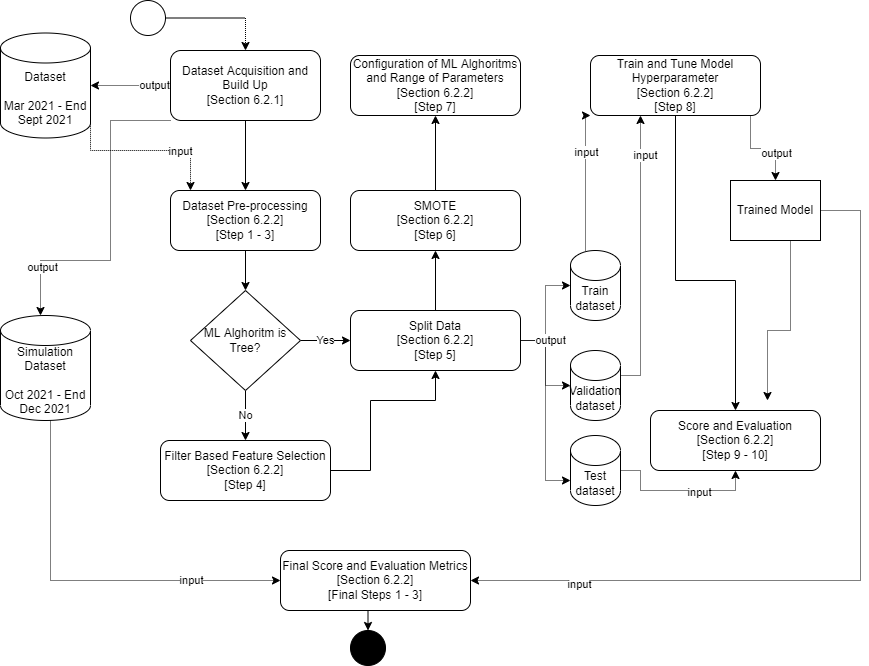
\includegraphics[width=\textwidth]{Chapters/Figures/DiagramaGeral.png}
	\caption{Diagram representing the experiment explained in the previous section.}
	\label{fig:Figuras_Tree_silhouettes-vectorial}
\end{figure}


\section{Results}

As stated earlier in our methodology, we will have two results per failure and asset to evaluate: the first one, that will evaluate our first test dataset and that contain the data from March 2021 to the final of September of 2021, and that will have represented all the failure events by using the stratified split on the fault category; the second one is a simulation of a real test of the model with a complete new dataset, that contains the data from October 2021 to the final of December 2021, and consequently, a complete set of failure events.

In the next subsections we will present for each fault and wind turbine, the model for each algorithm that presented the best result, with the parameters information that lead to that result.

%The complete list of results with all the parameters evaluation and that %lead us to the best machine learning model, will be represented in the %Appendix section, with the Appendix X.

Each scope is identified by three terms: the fault id, that indicates a identifier of the fault, the wind park id, with a three-letter string and the asset/wind turbine id, that is an identifier of the wind turbine of the park. These scopes are the ones presented in the Methodology section, in Table 5.3 and Table 5.4.

%DEPRECATED SINCE WE USE F1 SCORE IN THE TUNE MODEL HYPERPARAMETER
%We consider the best model by evaluating their metrics. As mentioned before, we prioritize the minimum %value of false positives and only then try to maximize the true positives. In terms of the precision, %recall, F1 score metrics, this means that we will prioritize the precision metric and then the F1 score %(that is balance of precision and recall).

The selection of the best model was made by evaluating their metrics. As mentioned before, we prioritize the minimum value of false positives, but we also want that our model is fitted to predict some failures.
So we will consider the F1 Score, as mentioned before in the Tune Model Hyperparameter module, as it evaluate the best balance between the precision and recall.

In each subsection we will have three tables with the evaluations:
\begin{enumerate}
    \item 
The first table will have the results of the first dataset, from 5th March 2021 to the final of September 2021, that was used to train, fit and tune the model. The results presented are from the test dataset and using the evaluate model module. We will use the evaluation metrics presented earlier in the methodology: precision, recall and F1 score.
    \item
The second table, presents the result of the simulation of running the already existing machine learning model with a new dataset, from October 2021 to the end of December 2021. In this table we will present the same metrics as in the previous step, also from the evaluate model module.
    \item
The final table, will present the results of our evaluation script, presented earlier in the methodology, and that tell us the real performance of the model by analyzing the confusion matrix metrics of the intervals of prediction that our model has predicted, as explained in the methodology section.
\end{enumerate}

In these subsections we will also present the best hyperparameters selected from the tune model hyperparameter module for each model and algorithm studied. The time window of these models are the ones presented in the third table presented earlier.

The number of fault events that exist for each of the fault and scope presented bellow was presented earlier in the subsection 5.4.

%VER SE NAO COLOCO TAMBEM O NRINTERVALOS, ETC

\subsection{Fault 9112 - SCA 34}

\begin{table}[!ht]
    \centering
    \begin{tabular}{|l|l|l|l|l|}
    \hline
        Algorithm & Time Window & Precision & Recall & F1 Score \\ \hline
        Two-Class Logistic Regression & 72 & 0.814 & 0.641 & 0.717 \\ \hline
        Two-Class Support Vector Machine & 24 & 0.553 & 0.698 & 0.617 \\ \hline
        Two-Class Neural Network & 72 & 0.849 & 0.857 & 0.853 \\ \hline
        Two-Class Decision Forest & 72 & 0.992 & 0.992 & 0.985 \\ \hline
        Two-Class Boosted Decision Tree & 72 & 0.99 & 0.995 & 0.992 \\ \hline
    \end{tabular}
    \caption{Fault 9112 - SCA 34: First Split (March 2021 - End September 2021) - Test Dataset - Evaluate Model Results}
    \label{9112_SCA34_1st}
\end{table}

\begin{table}[!ht]
    \centering
    \begin{tabular}{|l|l|l|l|l|}
    \hline
        Algorithm & Time Window & Precision & Recall & F1 Score \\ \hline
        Two-Class Logistic Regression & 12 & 0.341 & 0.279 & 0.307 \\ \hline
        Two-Class Support Vector Machine & 12 & 0.338 & 0.307 & 0.322 \\ \hline
        Two-Class Neural Network & 72 & 0.352 & 0.461 & 0.399 \\ \hline
        Two-Class Decision Forest & 72 & 0.391 & 0.45 & 0.418 \\ \hline
        Two-Class Boosted Decision Tree & 72 & 0.389 & 0.552 & 0.445 \\ \hline
    \end{tabular}
    \caption{Fault 9112 - SCA 34: Second Split (October 2021 - End December 2021) - Evaluate Model Results}
    \label{9112_SCA34_2nd}
\end{table}

\begin{table}[!ht]
    \centering
    \begin{tabular}{|l|l|l|l|l|l|}
    \hline
        Algorithm & Time Window & \% Threshold & FP & TP & FN \\ \hline
        Two-Class Logistic Regression & 24 & 0.2 & 0 & 15 & 3 \\ \hline
        Two-Class Support Vector Machine & 24 & 0.2 & 0 & 15 & 3 \\ \hline
        Two-Class Neural Network & 24 & 0.2 ; 0.3 & 0 & 16 & 2 \\ \hline
        Two-Class Decision Forest & 24 & 0.2 & 0 & 15 & 3 \\ \hline
        Two-Class Boosted Decision Tree & 24 & 0.2 & 0 & 15 & 3 \\ \hline
    \end{tabular}
	\caption{Fault 9112 - SCA 34: Second Split (October 2021 - End December 2021) - Evaluation Script Predictions}
    \label{9112_SCA34_3rd}
\end{table}

In terms of the machine learning model built for each algorithm that provided the best result on the final evaluation dataset, the best hyperparameters selected from the Tune Model Hyperparameter module are:

\begin{enumerate}
    \item{Two-Class Logistic Regression}
    
    \begin{enumerate}
        \item{Optimization Tolerance:} 0
        \item{Regularization Weight:} 1
    \end{enumerate}
    
    \item{Two-Class Support Vector Machine}
    
    \begin{enumerate}
        \item{Number of Iterations:} 750
        \item{Lambda:}[0.01, 0.001, 0.0001, 0.00001]
    \end{enumerate}
    
    \item{Two-Class Neural Network}
    
    \begin{enumerate}
        \item{Number of Learning Iterations:} 500
        \item{Learning Rate:}  0.4
    \end{enumerate}
    
    \item{Two-Class Decision Forest}

    \begin{enumerate}
        \item{Number of Decision Trees:} 32
        \item{Minimum number of samples per leaf node:} 1
        \item{Maximum depth of the decision tree:} 64
    \end{enumerate}
    
    \item{Two-Class Boosted Decision Tree}
    
    \begin{enumerate}
        \item{Maximum number of leaves per tree:} 128
        \item{Number of trees constructed:} 250
        \item{Minimum number of samples per leaf node:} 25
        \item{Learning Rate:}  0.6
    \end{enumerate}
    
\end{enumerate}


\subsection{Fault 8749 - PAP 35}

\begin{table}[!ht]
    \centering
    \begin{tabular}{|l|l|l|l|l|}
    \hline
        Algorithm & Time Window & Precision & Recall & F1 Score \\ \hline
        Two-Class Logistic Regression & 72 & 0.587 & 0.567 & 0.577 \\ \hline
        Two-Class Support Vector Machine & 72 & 0.515 & 0.465 & 0.489 \\ \hline
        Two-Class Neural Network & 72 & 0.975 & 0.985 & 0.98 \\ \hline
        Two-Class Decision Forest & 72 & 0.996 & 0.994 & 0.995 \\ \hline
        Two-Class Boosted Decision Tree & 72 & 0.999 & 0.994 & 0.997 \\ \hline
    \end{tabular}
    \caption{Fault 8749 - PAP 35: First Split (March 2021 - End September 2021) - Test Dataset - Evaluate Model Results}
    \label{9112_SCA34_1st}
\end{table}

\begin{table}[!ht]
    \centering
    \begin{tabular}{|l|l|l|l|l|}
    \hline
        Algorithm & Time Window & Precision & Recall & F1 Score \\ \hline
        Two-Class Logistic Regression & 72 & 0.288 & 0.16 & 0.206 \\ \hline
        Two-Class Support Vector Machine & 72 & 0.167 & 0.099 & 0.124 \\ \hline
        Two-Class Neural Network & 72 & 0.259 & 0.237 & 0.248 \\ \hline
        Two-Class Decision Forest & 72 & 0.223 & 0.369 & 0.278 \\ \hline
        Two-Class Boosted Decision Tree & 72 & 0.43 & 0.295 & 0.35 \\ \hline
    \end{tabular}
    \caption{Fault 8749 - PAP 35: Second Split (October 2021 - End December 2021) - Evaluate Model Results}
    \label{9112_SCA34_1st}
\end{table}

\begin{table}[!ht]
    \centering
    \begin{tabular}{|l|l|l|l|l|l|}
    \hline
        Algorithm & Time Window & \% Threshold & FP & TP & FN \\ \hline
        Two-Class Logistic Regression & 24 & 0.2 ; 0.3 & 0 & 2 & 6 \\ \hline
        Two-Class Support Vector Machine & 72 & 0.2 ; 0.3 & 0 & 1 & 7 \\ \hline
        Two-Class Neural Network & 72 & 0.2 & 0 & 2 & 6 \\ \hline
        Two-Class Decision Forest & 72 & 0.4 ; 0.5 ; 0.6 & 0 & 1 & 7 \\ \hline
        Two-Class Boosted Decision Tree & 72 & 0.5 ; 0.6 ; 0.7 & 0 & 1 & 7 \\ \hline
    \end{tabular}
    \caption{Fault 8749 - PAP 35: Second Split (October 2021 - End December 2021) - Evaluation Script Predictions}
    \label{9112_SCA34_1st}
\end{table}

In terms of the machine learning model built for each algorithm, the best hyperparameters selected from the Tune Model Hyperparameter module are:

\begin{enumerate}
    \item{Two-Class Logistic Regression}
    
    \begin{enumerate}
        \item{Optimization Tolerance:} 0
        \item{Regularization Weight:} 0.01
    \end{enumerate}
    
    \item{Two-Class Support Vector Machine}
    
    \begin{enumerate}
        \item{Number of Iterations:} 750
        \item{Lambda:} All
    \end{enumerate}
    
    \item{Two-Class Neural Network}
    
    \begin{enumerate}
        \item{Number of Learning Iterations:} 500
        \item{Learning Rate:}  0.6
    \end{enumerate}
    
    \item{Two-Class Decision Forest}

    \begin{enumerate}
        \item{Number of Decision Trees:} 32
        \item{Minimum number of samples per leaf node:} 1
        \item{Maximum depth of the decision tree:} [32, 64]
    \end{enumerate}
    
    \item{Two-Class Boosted Decision Tree}
    
    \begin{enumerate}
        \item{Maximum number of leaves per tree:} [64,128]
        \item{Number of trees constructed:} 500
        \item{Minimum number of samples per leaf node:} 10,50
        \item{Learning Rate:} [0.2, 0.1]
    \end{enumerate}
    
\end{enumerate}


\subsection{Fault 768 - BNE 18}

\begin{table}[!ht]
    \centering
    \begin{tabular}{|l|l|l|l|l|}
    \hline
        Algorithm & Time Window & Precision & Recall & F1 Score \\ \hline
        Two-Class Logistic Regression & 72 & 0.447 & 0.224 & 0.298 \\ \hline
        Two-Class Support Vector Machine & 72 & 0.875 & 0.082 & 0.151 \\ \hline
        Two-Class Neural Network & 24 & 0.966 & 1 & 0.983 \\ \hline
        Two-Class Decision Forest & 72 & 0.998 & 0.993 & 0.995 \\ \hline
        Two-Class Boosted Decision Tree & 72 & 1 & 0.993 & 0.996 \\ \hline
    \end{tabular}
    \caption{Fault 768 - BNE 18: First Split (March 2021 - End September 2021) - Test Dataset - Evaluate Model Results}
    \label{9112_SCA34_1st}
\end{table}

\begin{table}[!ht]
    \centering
    \begin{tabular}{|l|l|l|l|l|}
    \hline
        Algorithm & Time Window & Precision & Recall & F1 Score \\ \hline
        Two-Class Logistic Regression & 72 & 0.126 & 0.02 & 0.035 \\ \hline
        Two-Class Support Vector Machine & All & 1 & 0 & 0 \\ \hline
        Two-Class Neural Network & 72 & 0.291 & 0.066 & 0.107 \\ \hline
        Two-Class Decision Forest & 72 & 0.481 & 0.116 & 0.187 \\ \hline
        Two-Class Boosted Decision Tree & 72 & 0.42 & 0.114 & 0.179 \\ \hline
    \end{tabular}
    \caption{Fault 768 - BNE 18: Second Split (October 2021 - End December 2021) - Test Dataset - Evaluate Model Results}
    \label{9112_SCA34_1st}
\end{table}

\begin{table}[!ht]
    \centering
    \begin{tabular}{|l|l|l|l|l|l|}
    \hline
        Algorithm & Time Window & \% Threshold & FP & TP & FN \\ \hline
        Two-Class Logistic Regression & All & All & 0 & 0 & 8 \\ \hline
        Two-Class Support Vector Machine & All & All & 0 & 0 & 8 \\ \hline
        Two-Class Neural Network & 72 & >= 0.4 & 0 & 0 & 8 \\ \hline
        Two-Class Decision Forest & 72 & 0.2 & 0 & 1 & 7 \\ \hline
        Two-Class Boosted Decision Tree & 72 & 0.2 & 0 & 1 & 7 \\ \hline
    \end{tabular}
    \caption{Fault 768 - BNE 18: Second Split (October 2021 - End December 2021) - Evaluation Script Predictions}
    \label{9112_SCA34_1st}
\end{table}

In terms of the machine learning model built for each algorithm, the best hyperparameters selected from the Tune Model Hyperparameter module are:

\begin{enumerate}
    \item{Two-Class Logistic Regression}
    
    \begin{enumerate}
        \item{Optimization Tolerance:} 0
        \item{Regularization Weight:} 0.01
    \end{enumerate}
    
    \item{Two-Class Support Vector Machine}
    
    \begin{enumerate}
        \item{Number of Iterations:} 750
        \item{Lambda:} All
    \end{enumerate}
    
    \item{Two-Class Neural Network}
    
    \begin{enumerate}
        \item{Number of Learning Iterations:} 160
        \item{Learning Rate:} 0.8
    \end{enumerate}
    
    \item{Two-Class Decision Forest}

    \begin{enumerate}
        \item{Number of Decision Trees:} 16
        \item{Minimum number of samples per leaf node:} 1
        \item{Maximum depth of the decision tree:} 32
    \end{enumerate}
    
    \item{Two-Class Boosted Decision Tree}
    For this model, the Tune Model Hyperparameter module return almost all the parameter range values as classified with the same ranking. So it is not possible to take conclusions on the hyperparameters that provided the best results
    
\end{enumerate}


\subsection{Fault 768 - CHF 28}

\begin{table}[!ht]
    \centering
    \begin{tabular}{|l|l|l|l|l|}
    \hline
        Algorithm & Time Window & Precision & Recall & F1 Score \\ \hline
        Two-Class Logistic Regression & 12 & 0.561 & 0.217 & 0.313 \\ \hline
        Two-Class Support Vector Machine & 72 & 0.561 & 0.107 & 0.18 \\ \hline
        Two-Class Neural Network & 12 & 0.991 & 0.991 & 0.991 \\ \hline
        Two-Class Decision Forest & 72 & 0.999 & 1 & 0.999 \\ \hline
        Two-Class Boosted Decision Tree & 72 & 0.999 & 1 & 0.999 \\ \hline
    \end{tabular}
    \caption{Fault 768 - CHF 28: First Split (March 2021 - End September 2021) - Test Dataset - Evaluate Model Results}
    \label{9112_SCA34_1st}
\end{table}

\begin{table}[!ht]
    \centering
    \begin{tabular}{|l|l|l|l|l|}
    \hline
        Algorithm & Time Window & Precision & Recall & F1 Score \\ \hline
        Two-Class Logistic Regression & 72 & 0.7 & 0.161 & 0.262 \\ \hline
        Two-Class Support Vector Machine & 72 & 0.81 & 0.074 & 0.136 \\ \hline
        Two-Class Neural Network & 72 & 0.444 & 0.123 & 0.193 \\ \hline
        Two-Class Decision Forest & 72 & 0.681 & 0.11 & 0.189 \\ \hline
        Two-Class Boosted Decision Tree & 72 & 0.651 & 0.084 & 0.148 \\ \hline
    \end{tabular}
    \caption{Fault 768 - CHF 28: Second Split (October 2021 - End December 2021) - Evaluate Model Results - Test Dataset - Evaluate Model Results}
    \label{9112_SCA34_1st}
\end{table}

\begin{table}[!ht]
    \centering
    \begin{tabular}{|l|l|l|l|l|l|}
    \hline
        Algorithm & Time Window & \% Threshold & FP & TP & FN \\ \hline
        Two-Class Logistic Regression & 72 & 0.2 & 0 & 21 & 3 \\ \hline
        Two-Class Support Vector Machine & 72 & 0.2 & 0 & 10 & 14 \\ \hline
        Two-Class Neural Network & 12, 72 & 0.2 & 0 & 2 & 22 \\ \hline
        Two-Class Decision Forest & 72 & 0.2 & 0 & 8 & 16 \\ \hline
        Two-Class Boosted Decision Tree & 72 & 0.2 & 0 & 1 & 23 \\ \hline
    \end{tabular}
    \caption{Fault 768 - CHF 28: Second Split (October 2021 - End December 2021) - Evaluation Script Predictions}
    \label{9112_SCA34_1st}
\end{table}

In terms of the machine learning model built for each algorithm, the best hyperparameters selected from the Tune Model Hyperparameter module are:

\begin{enumerate}
    \item{Two-Class Logistic Regression}
    
    \begin{enumerate}
        \item{Optimization Tolerance:} 0
        \item{Regularization Weight:} 0.1
    \end{enumerate}
    
    \item{Two-Class Support Vector Machine}
    
    \begin{enumerate}
        \item{Number of Iterations:} 750
        \item{Lambda:} All
    \end{enumerate}
    
    \item{Two-Class Neural Network}
    
    \begin{enumerate}
        \item{Number of Learning Iterations:} 500
        \item{Learning Rate:} 0.6
    \end{enumerate}
    
    \item{Two-Class Decision Forest}

    \begin{enumerate}
        \item{Number of Decision Trees:} 32
        \item{Minimum number of samples per leaf node:} 1
        \item{Maximum depth of the decision tree:} [32, 64]
    \end{enumerate}
    
    \item{Two-Class Boosted Decision Tree}
    
    \begin{enumerate}
        \item{Maximum number of leaves per tree:} [128,64]
        \item{Number of trees constructed:} [50, 500, 250]
        \item{Minimum number of samples per leaf node:} [10,1]
        \item{Learning Rate:} All
    \end{enumerate}
    
\end{enumerate}


\subsection{Fault 140 - PCA 7}

\begin{table}[!ht]
    \centering
    \begin{tabular}{|l|l|l|l|l|}
    \hline
        Algorithm & Time Window & Precision & Recall & F1 Score \\ \hline
        Two-Class Logistic Regression & 72 & 0.587 & 0.556 & 0.571 \\ \hline
        Two-Class Support Vector Machine & 72 & 0.598 & 0.542 & 0.569 \\ \hline
        Two-Class Neural Network & 72 & 0.978 & 0.978 & 0.978 \\ \hline
        Two-Class Decision Forest & 72 & 0.996 & 0.995 & 0.996 \\ \hline
        Two-Class Boosted Decision Tree & 24 & 0.999 & 0.997 & 0.998 \\ \hline
    \end{tabular}
    \caption{Fault 140 - PCA 7: First Split (March 2021 - End September 2021) - Test Dataset - Evaluate Model Results}
    \label{9112_SCA34_1st}
\end{table}

\begin{table}[!ht]
    \centering
    \begin{tabular}{|l|l|l|l|l|}
    \hline
        Algorithm & Time Window & Precision & Recall & F1 Score \\ \hline
        Two-Class Logistic Regression & 72 & 0.139 & 0.571 & 0.223 \\ \hline
        Two-Class Support Vector Machine & 72 & 0.141 & 0.579 & 0.227 \\ \hline
        Two-Class Neural Network & 72 & 0.124 & 0.546 & 0.202 \\ \hline
        Two-Class Decision Forest & 72 & 0.129 & 0.42 & 0.197 \\ \hline
        Two-Class Boosted Decision Tree & 72 & 0.146 & 0.262 & 0.188 \\ \hline
    \end{tabular}
    \caption{Fault 140 - PCA 7: Second Split (October 2021 - End December 2021) - Evaluate Model Results}
    \label{9112_SCA34_1st}
\end{table}

\begin{table}[!ht]
    \centering
    \begin{tabular}{|l|l|l|l|l|l|}
    \hline
        Algorithm & Time Window & \% Threshold & FP & TP & FN \\ \hline
        Two-Class Logistic Regression & 72 & 0.3, 0.4, 0.5 & 0 & 11 & 2 \\ \hline
        Two-Class Support Vector Machine & 72 & 0.3, 0.4, 0.5 & 0 & 11 & 2 \\ \hline
        Two-Class Neural Network & 72 & 0.3 & 0 & 11 & 2 \\ \hline
        Two-Class Decision Forest & 72 & 0.2 & 0 & 10 & 3 \\ \hline
        Two-Class Boosted Decision Tree & 12 & <= 0.6 & 0 & 2 & 11 \\ \hline
    \end{tabular}
    \caption{Fault 140 - PCA 7: Second Split (October 2021 - End December 2021) - Evaluation Script Predictions}
    \label{9112_SCA34_1st}
\end{table}

In terms of the machine learning model built for each algorithm, the best hyperparameters selected from the Tune Model Hyperparameter module are:

\begin{enumerate}
    \item{Two-Class Logistic Regression}
    
    \begin{enumerate}
        \item{Optimization Tolerance:} 0
        \item{Regularization Weight:} 0.1
    \end{enumerate}
    
    \item{Two-Class Support Vector Machine}
    
    \begin{enumerate}
        \item{Number of Iterations:} 100
        \item{Lambda:} All
    \end{enumerate}
    
    \item{Two-Class Neural Network}
    
    \begin{enumerate}
        \item{Number of Learning Iterations:} 500
        \item{Learning Rate:} 0.4
    \end{enumerate}
    
    \item{Two-Class Decision Forest}

    \begin{enumerate}
        \item{Number of Decision Trees:} 16
        \item{Minimum number of samples per leaf node:} 1
        \item{Maximum depth of the decision tree:} 32
    \end{enumerate}
    
    \item{Two-Class Boosted Decision Tree}
    
    \begin{enumerate}
        \item{Maximum number of leaves per tree:} 128
        \item{Number of trees constructed:} [50, 100]
        \item{Minimum number of samples per leaf node:} 10
        \item{Learning Rate:} 0.4
    \end{enumerate}
    
\end{enumerate}


\subsection{Fault 14474 - TMS 6}

\begin{table}[!ht]
    \centering
    \begin{tabular}{|l|l|l|l|l|}
    \hline
        Algorithm & Time Window & Precision & Recall & F1 Score \\ \hline
        Two-Class Logistic Regression & 72 & 0.414 & 0.317 & 0.359 \\ \hline
        Two-Class Support Vector Machine & 72 & 0.574 & 0.14 & 0.224 \\ \hline
        Two-Class Neural Network & 72 & 0.939 & 0.943 & 0.941 \\ \hline
        Two-Class Decision Forest & 72 & 0.998 & 0.99 & 0.994 \\ \hline
        Two-Class Boosted Decision Tree & 72 & 0.999 & 0.993 & 0.996 \\ \hline
    \end{tabular}
    \caption{Fault 14474 - TMS 6: First Split (March 2021 - End September 2021) - Test Dataset - Evaluate Model Results}
    \label{9112_SCA34_1st}
\end{table}

\begin{table}[!ht]
    \centering
    \begin{tabular}{|l|l|l|l|l|}
    \hline
        Algorithm & Time Window & Precision & Recall & F1 Score \\ \hline
        Two-Class Logistic Regression & 72 & 0.399 & 0.073 & 0.124 \\ \hline
        Two-Class Support Vector Machine & 72 & 0.265 & 0.018 & 0.033 \\ \hline
        Two-Class Neural Network & 72 & 0.173 & 0.083 & 0.112 \\ \hline
        Two-Class Decision Forest & 24 & 0.62 & 0.228 & 0.333 \\ \hline
        Two-Class Boosted Decision Tree & 72 & 0.05 & 0.009 & 0.015 \\ \hline
    \end{tabular}
    \caption{Fault 14474 - TMS 6: Second Split (October 2021 - End December 2021) - Evaluate Model Results}
    \label{9112_SCA34_1st}
\end{table}

\begin{table}[!ht]
    \centering
    \begin{tabular}{|l|l|l|l|l|l|}
    \hline
        Algorithm & Time Window & \% Threshold & FP & TP & FN \\ \hline
        Two-Class Logistic Regression & 12, 72 & >= 0.3 & 0 & 0 & 10 \\ \hline
        Two-Class Support Vector Machine & All & All & 0 & 0 & 10 \\ \hline
        Two-Class Neural Network & 72 & >= 0.3 & 0 & 0 & 10 \\ \hline
        Two-Class Decision Forest & 12, 24 & All & 0 & 0 & 10 \\ \hline
        Two-Class Boosted Decision Tree & 12, 24 & All & 0 & 0 & 10 \\ \hline
    \end{tabular}
    \caption{Fault 14474 - TMS 6: Second Split (October 2021 - End December 2021) - Evaluation Script Predictions}
    \label{9112_SCA34_1st}
\end{table}

In terms of the machine learning model built for each algorithm, the best hyperparameters selected from the Tune Model Hyperparameter module are:

\begin{enumerate}
    \item{Two-Class Logistic Regression}
    
    \begin{enumerate}
        \item{Optimization Tolerance:} 0
        \item{Regularization Weight:} 0.01
    \end{enumerate}
    
    \item{Two-Class Support Vector Machine}
    
    \begin{enumerate}
        \item{Number of Iterations:} 750
        \item{Lambda:} All
    \end{enumerate}
    
    \item{Two-Class Neural Network}
    
    \begin{enumerate}
        \item{Number of Learning Iterations:} 500
        \item{Learning Rate:} 0.4
    \end{enumerate}
    
    \item{Two-Class Decision Forest}

    \begin{enumerate}
        \item{Number of Decision Trees:} 16
        \item{Minimum number of samples per leaf node:} 1
        \item{Maximum depth of the decision tree:} 16
    \end{enumerate}
    
    \item{Two-Class Boosted Decision Tree}
    
    \begin{enumerate}
        \item{Maximum number of leaves per tree:} 32
        \item{Number of trees constructed:} 500
        \item{Minimum number of samples per leaf node:} 1
        \item{Learning Rate:} 0.05
    \end{enumerate}
    
\end{enumerate}


\subsection{Fault 768 - BNE 14}

\begin{table}[!ht]
    \centering
    \begin{tabular}{|l|l|l|l|l|}
    \hline
        Algorithm & Time Window & Precision & Recall & F1 Score \\ \hline
        Two-Class Logistic Regression & 24 & 0.555 & 0.233 & 0.328 \\ \hline
        Two-Class Support Vector Machine & 24 & 0.636 & 0.119 & 0.2 \\ \hline
        Two-Class Neural Network & 72 & 0.986 & 0.99 & 0.988 \\ \hline
        Two-Class Decision Forest & 72 & 1 & 0.991 & 0.996 \\ \hline
        Two-Class Boosted Decision Tree & 72 & 1 & 0.995 & 0.998 \\ \hline
    \end{tabular}
    \caption{Fault 768 - BNE 14: First Split (March 2021 - End September 2021) - Test Dataset - Evaluate Model Results}
    \label{9112_SCA34_1st}
\end{table}

\begin{table}[!ht]
    \centering
    \begin{tabular}{|l|l|l|l|l|}
    \hline
        Algorithm & Time Window & Precision & Recall & F1 Score \\ \hline
        Two-Class Logistic Regression & All & 0 & 0 & 0 \\ \hline
        Two-Class Support Vector Machine & All & 0 & 0 & 0 \\ \hline
        Two-Class Neural Network & All & 0 & 0 & 0 \\ \hline
        Two-Class Decision Forest & All & 0 & 0 & 0 \\ \hline
        Two-Class Boosted Decision Tree & All & 0 & 0 & 0 \\ \hline
    \end{tabular}
    \caption{Fault 768 - BNE 14: Second Split (October 2021 - End December 2021) - Evaluate Model Results}
    \label{9112_SCA34_1st}
\end{table}

\begin{table}[!ht]
    \centering
    \begin{tabular}{|l|l|l|l|l|l|}
    \hline
        Algorithm & Time Window & \% Threshold & FP & TP & FN \\ \hline
        Two-Class Logistic Regression & All & All & 0 & 0 & 6 \\ \hline
        Two-Class Support Vector Machine & 12, 72 & All & 0 & 0 & 6 \\ \hline
        Two-Class Neural Network & All & All & 0 & 0 & 6 \\ \hline
        Two-Class Decision Forest & All & All & 0 & 0 & 6 \\ \hline
        Two-Class Boosted Decision Tree & All & All & 0 & 0 & 6 \\ \hline
    \end{tabular}
    \caption{Fault 768 - BNE 14: Second Split (October 2021 - End December 2021) - Evaluation Script Predictions}
    \label{9112_SCA34_1st}
\end{table}

In terms of the machine learning model built for each algorithm, the best hyperparameters selected from the Tune Model Hyperparameter module are:

\begin{enumerate}
    \item{Two-Class Logistic Regression}
    
    \begin{enumerate}
        \item{Optimization Tolerance:} 0
        \item{Regularization Weight:} 0.01
    \end{enumerate}
    
    \item{Two-Class Support Vector Machine}
    
    \begin{enumerate}
        \item{Number of Iterations:} 750
        \item{Lambda:} All
    \end{enumerate}
    
    \item{Two-Class Neural Network}
    
    \begin{enumerate}
        \item{Number of Learning Iterations:} 500
        \item{Learning Rate:} 0.4
    \end{enumerate}
    
    \item{Two-Class Decision Forest}

    \begin{enumerate}
        \item{Number of Decision Trees:} 32
        \item{Minimum number of samples per leaf node:} 1
        \item{Maximum depth of the decision tree:} [32,64]
    \end{enumerate}
    
    \item{Two-Class Boosted Decision Tree}
    
    \begin{enumerate}
        \item{Maximum number of leaves per tree:} [32, 64, 128]
        \item{Number of trees constructed:} [250,500]
        \item{Minimum number of samples per leaf node:} All
        \item{Learning Rate:} All
    \end{enumerate}
    
\end{enumerate}


\subsection{Fault 367 - CHF 15}

\begin{table}[!ht]
    \centering
    \begin{tabular}{|l|l|l|l|l|}
    \hline
        Algorithm & Time Window & Precision & Recall & F1 Score \\ \hline
        Two-Class Logistic Regression & 72 & 0.32 & 0.068 & 0.111 \\ \hline
        Two-Class Support Vector Machine & 72 & 0.471 & 0.034 & 0.063 \\ \hline
        Two-Class Neural Network & 24 & 0.979 & 0.979 & 0.979 \\ \hline
        Two-Class Decision Forest & 72 & 1 & 0.992 & 0.996 \\ \hline
        Two-Class Boosted Decision Tree & 72 & 0.998 & 0.994 & 0.996 \\ \hline
    \end{tabular}
    \caption{Fault 367 - CHF 15: First Split (March 2021 - End September 2021) - Test Dataset - Evaluate Model Results}
    \label{9112_SCA34_1st}
\end{table}

\begin{table}[!ht]
    \centering
    \begin{tabular}{|l|l|l|l|l|}
    \hline
        Algorithm & Time Window & Precision & Recall & F1 Score \\ \hline
        Two-Class Logistic Regression & 72 & 0.6 & 0.052 & 0.095 \\ \hline
        Two-Class Support Vector Machine & All & 1 & 0 & 0 \\ \hline
        Two-Class Neural Network & 72 & 0.154 & 0.063 & 0.089 \\ \hline
        Two-Class Decision Forest & 72 & 0.12 & 0.029 & 0.046 \\ \hline
        Two-Class Boosted Decision Tree & 72 & 0.104 & 0.031 & 0.048 \\ \hline
    \end{tabular}
    \caption{Fault 367 - CHF 15: Second Split (October 2021 - End December 2021) - Evaluate Model Results}
    \label{9112_SCA34_1st}
\end{table}

\begin{table}[!ht]
    \centering
    \begin{tabular}{|l|l|l|l|l|l|}
    \hline
        Algorithm & Time Window & \% Threshold & FP & TP & FN \\ \hline
        Two-Class Logistic Regression & 24, 72 & All & 0 & 0 & 4 \\ \hline
        Two-Class Support Vector Machine & All & All & 0 & 0 & 4 \\ \hline
        Two-Class Neural Network & 24, 72 & All & 0 & 0 & 4 \\ \hline
        Two-Class Decision Forest & All & All & 0 & 0 & 4 \\ \hline
        Two-Class Boosted Decision Tree & 12, 24 & All & 0 & 0 & 4 \\ \hline
    \end{tabular}
    \caption{Fault 367 - CHF 15: Second Split (October 2021 - End December 2021) - Evaluation Script Predictions}
    \label{9112_SCA34_1st}
\end{table}

In terms of the machine learning model built for each algorithm, the best hyperparameters selected from the Tune Model Hyperparameter module are:

\begin{enumerate}
    \item{Two-Class Logistic Regression}
    
    \begin{enumerate}
        \item{Optimization Tolerance:} 0
        \item{Regularization Weight:} 0.1
    \end{enumerate}
    
    \item{Two-Class Support Vector Machine}
    
    \begin{enumerate}
        \item{Number of Iterations:} 750
        \item{Lambda:} All
    \end{enumerate}
    
    \item{Two-Class Neural Network}
    
    \begin{enumerate}
        \item{Number of Learning Iterations:} 500
        \item{Learning Rate:} 0.2
    \end{enumerate}
    
    \item{Two-Class Decision Forest}

    \begin{enumerate}
        \item{Number of Decision Trees:} 32
        \item{Minimum number of samples per leaf node:} 1
        \item{Maximum depth of the decision tree:} [32,64]
    \end{enumerate}

    \item{Two-Class Boosted Decision Tree}
    
    \begin{enumerate}
        \item{Maximum number of leaves per tree:} 8
        \item{Number of trees constructed:} 250
        \item{Minimum number of samples per leaf node:} 25
        \item{Learning Rate:} 0.2
    \end{enumerate}
    
\end{enumerate}


\subsection{Fault 140 - PLS 9}

\begin{table}[!ht]
    \centering
    \begin{tabular}{|l|l|l|l|l|}
    \hline
        Algorithm & Time Window & Precision & Recall & F1 Score \\ \hline
        Two-Class Logistic Regression & 72 & 0.469 & 0.374 & 0.416 \\ \hline
        Two-Class Support Vector Machine & 72 & 0.48 & 0.359 & 0.411 \\ \hline
        Two-Class Neural Network & 72 & 0.964 & 0.98 & 0.972 \\ \hline
        Two-Class Decision Forest & 72 & 0.993 & 0.992 & 0.993 \\ \hline
        Two-Class Boosted Decision Tree & 72 & 0.996 & 0.997 & 0.997 \\ \hline
    \end{tabular}
    \caption{Fault 140 - PLS 9: First Split (March 2021 - End September 2021) - Test Dataset - Evaluate Model Results}
    \label{9112_SCA34_1st}
\end{table}

\begin{table}[!ht]
    \centering
    \begin{tabular}{|l|l|l|l|l|}
    \hline
        Algorithm & Time Window & Precision & Recall & F1 Score \\ \hline
        Two-Class Logistic Regression & 72 & 0.098 & 0.394 & 0.156 \\ \hline
        Two-Class Support Vector Machine & 72 & 0.096 & 0.398 & 0.155 \\ \hline
        Two-Class Neural Network & 72 & 0.077 & 0.194 & 0.111 \\ \hline
        Two-Class Decision Forest & 72 & 0.064 & 0.17 & 0.093 \\ \hline
        Two-Class Boosted Decision Tree & 72 & 0.066 & 0.17 & 0.095 \\ \hline
    \end{tabular}
    \caption{Fault 140 - PLS 9: Second Split (October 2021 - End December 2021) - Evaluate Model Results}
    \label{9112_SCA34_1st}
\end{table}

\begin{table}[!ht]
    \centering
    \begin{tabular}{|l|l|l|l|l|l|}
    \hline
        Algorithm & Time Window & \% Threshold & FP & TP & FN \\ \hline
        Two-Class Logistic Regression & 12, 24 & All & 0 & 0 & 3 \\ \hline
        Two-Class Support Vector Machine & 24 & All & 0 & 0 & 3 \\ \hline
        Two-Class Neural Network & 12 & <= 0.4 & 0 & 1 & 2 \\ \hline
        Two-Class Decision Forest & 12, 24 & All & 0 & 0 & 3 \\ \hline
        Two-Class Boosted Decision Tree & 12 & All & 0 & 0 & 3 \\ \hline
    \end{tabular}
    \caption{Fault 140 - PLS 9: Second Split (October 2021 - End December 2021) - Evaluation Script Predictions}
    \label{9112_SCA34_1st}
\end{table}

In terms of the machine learning model built for each algorithm, the best hyperparameters selected from the Tune Model Hyperparameter module are:

\begin{enumerate}
    \item{Two-Class Logistic Regression}
    
    \begin{enumerate}
        \item{Optimization Tolerance:} 0
        \item{Regularization Weight:} 0.01
    \end{enumerate}
    
    \item{Two-Class Support Vector Machine}
    
    \begin{enumerate}
        \item{Number of Iterations:} 500
        \item{Lambda:} All
    \end{enumerate}
    
    \item{Two-Class Neural Network}
    
    \begin{enumerate}
        \item{Number of Learning Iterations:} 500
        \item{Learning Rate:} 0.6
    \end{enumerate}
    
    \item{Two-Class Decision Forest}

    \begin{enumerate}
        \item{Number of Decision Trees:} 16
        \item{Minimum number of samples per leaf node:} 1
        \item{Maximum depth of the decision tree:} 32
    \end{enumerate}
    
    \item{Two-Class Boosted Decision Tree}1
    
    \begin{enumerate}
        \item{Maximum number of leaves per tree:} 8
        \item{Number of trees constructed:} 500
        \item{Minimum number of samples per leaf node:} 10
        \item{Learning Rate:} 0.4
    \end{enumerate}
    
\end{enumerate}


\subsection{Fault 8487 - SCA 10}

\begin{table}[!ht]
    \centering
    \begin{tabular}{|l|l|l|l|l|}
    \hline
        Algorithm & Time Window & Precision & Recall & F1 Score \\ \hline
        Two-Class Logistic Regression & 24 & 0.688 & 0.543 & 0.607 \\ \hline
        Two-Class Support Vector Machine & 72 & 0.619 & 0.548 & 0.581 \\ \hline
        Two-Class Neural Network & 72 & 0.982 & 0.989 & 0.986 \\ \hline
        Two-Class Decision Forest & 24 & 0.99 & 0.996 & 0.993 \\ \hline
        Two-Class Boosted Decision Tree & 24 & 0.995 & 0.999 & 0.997 \\ \hline
    \end{tabular}
    \caption{Fault 8487 - SCA 10: First Split (March 2021 - End September 2021) - Test Dataset - Evaluate Model Results}
    \label{9112_SCA34_1st}
\end{table}

\begin{table}[!ht]
    \centering
    \begin{tabular}{|l|l|l|l|l|}
    \hline
        Algorithm & Time Window & Precision & Recall & F1 Score \\ \hline
        Two-Class Logistic Regression & All & 0 & 0 & 0 \\ \hline
        Two-Class Support Vector Machine & All & 0 & 0 & 0 \\ \hline
        Two-Class Neural Network & All & 0 & 0 & 0 \\ \hline
        Two-Class Decision Forest & All & 0 & 0 & 0 \\ \hline
        Two-Class Boosted Decision Tree & All & 0 & 0 & 0 \\ \hline
    \end{tabular}
    \caption{Fault 8487 - SCA 10: Second Split (October 2021 - End December 2021) - Evaluate Model Results}
    \label{9112_SCA34_1st}
\end{table}

\begin{table}[!ht]
    \centering
    \begin{tabular}{|l|l|l|l|l|l|}
    \hline
        Algorithm & Time Window & \% Threshold & FP & TP & FN \\ \hline
        Two-Class Logistic Regression & All & All & 0 & 0 & 0 \\ \hline
        Two-Class Support Vector Machine & All & All & 0 & 0 & 0 \\ \hline
        Two-Class Neural Network & All & All & 0 & 0 & 0 \\ \hline
        Two-Class Decision Forest & All & All & 0 & 0 & 0 \\ \hline
        Two-Class Boosted Decision Tree & All & All & 0 & 0 & 0 \\ \hline
    \end{tabular}
    \caption{Fault 8487 - SCA 10: Second Split (October 2021 - End December 2021) - Evaluation Script Predictions}
    \label{9112_SCA34_1st}
\end{table}

In terms of the machine learning model built for each algorithm, the best hyperparameters selected from the Tune Model Hyperparameter module are:

\begin{enumerate}
    \item{Two-Class Logistic Regression}24
    
    \begin{enumerate}
        \item{Optimization Tolerance:} 0
        \item{Regularization Weight:} 0.1
    \end{enumerate}
    
    \item{Two-Class Support Vector Machine}
    
    \begin{enumerate}
        \item{Number of Iterations:} 750
        \item{Lambda:} All
    \end{enumerate}
    
    \item{Two-Class Neural Network}
    
    \begin{enumerate}
        \item{Number of Learning Iterations:} 500
        \item{Learning Rate:} 0.6
    \end{enumerate}
    
    \item{Two-Class Decision Forest}

    \begin{enumerate}
        \item{Number of Decision Trees:} 32
        \item{Minimum number of samples per leaf node:} 1
        \item{Maximum depth of the decision tree:} [32,64]
    \end{enumerate}
    
    \item{Two-Class Boosted Decision Tree}
    
    \begin{enumerate}
        \item{Maximum number of leaves per tree:} 32
        \item{Number of trees constructed:} 500
        \item{Minimum number of samples per leaf node:} 1
        \item{Learning Rate:} 0.05
    \end{enumerate}
    
\end{enumerate}


\subsection{Fault 8719 - SCA 28}

\begin{table}[!ht]
    \centering
    \begin{tabular}{|l|l|l|l|l|}
    \hline
        Algorithm & Time Window & Precision & Recall & F1 Score \\ \hline
        Two-Class Logistic Regression & 72 & 0.414 & 0.317 & 0.359 \\ \hline
        Two-Class Support Vector Machine & 72 & 0.475 & 0.251 & 0.328 \\ \hline
        Two-Class Neural Network & 24 & 0.692 & 0.911 & 0.786 \\ \hline
        Two-Class Decision Forest & 72 & 0.996 & 0.997 & 0.996 \\ \hline
        Two-Class Boosted Decision Tree & 72 & 0.999 & 0.998 & 0.998 \\ \hline
    \end{tabular}
    \caption{Fault 8719 - SCA 28: First Split (March 2021 - End September 2021) - Test Dataset - Evaluate Model Results}
    \label{9112_SCA34_1st}
\end{table}

\begin{table}[!ht]
    \centering
    \begin{tabular}{|l|l|l|l|l|}
    \hline
        Algorithm & Time Window & Precision & Recall & F1 Score \\ \hline
        Two-Class Logistic Regression & All & 0 & 0 & 0 \\ \hline
        Two-Class Support Vector Machine & All & 0 & 0 & 0 \\ \hline
        Two-Class Neural Network & All & 0 & 0 & 0 \\ \hline
        Two-Class Decision Forest & All & 0 & 0 & 0 \\ \hline
        Two-Class Boosted Decision Tree & All & 0 & 0 & 0 \\ \hline
    \end{tabular}
    \caption{Fault 8719 - SCA 28: Second Split (October 2021 - End December 2021) - Evaluate Model Results}
    \label{9112_SCA34_1st}
\end{table}

\begin{table}[!ht]
    \centering
    \begin{tabular}{|l|l|l|l|l|l|}
    \hline
        Algorithm & Time Window & \% Threshold & FP & TP & FN \\ \hline
        Two-Class Logistic Regression & All & All & 0 & 0 & 0 \\ \hline
        Two-Class Support Vector Machine & All & All & 0 & 0 & 0 \\ \hline
        Two-Class Neural Network & All & All & 0 & 0 & 0 \\ \hline
        Two-Class Decision Forest & All & All & 0 & 0 & 0 \\ \hline
        Two-Class Boosted Decision Tree & All & All & 0 & 0 & 0 \\ \hline
    \end{tabular}
    \caption{Fault 8719 - SCA 28: Second Split (October 2021 - End December 2021) - Evaluation Script Predictions}
    \label{9112_SCA34_1st}
\end{table}

In terms of the machine learning model built for each algorithm, the best hyperparameters selected from the Tune Model Hyperparameter module are:

\begin{enumerate}
    \item{Two-Class Logistic Regression}
    
    \begin{enumerate}
        \item{Optimization Tolerance:} 0
        \item{Regularization Weight:} 0.01
    \end{enumerate}
    
    \item{Two-Class Support Vector Machine}
    
    \begin{enumerate}
        \item{Number of Iterations:} 750
        \item{Lambda:} 0.01x
    \end{enumerate}
    
    \item{Two-Class Neural Network}24
    
    \begin{enumerate}
        \item{Number of Learning Iterations:} 500
        \item{Learning Rate:} 0.6
    \end{enumerate}
    
    \item{Two-Class Decision Forest}

    \begin{enumerate}
        \item{Number of Decision Trees:} 32
        \item{Minimum number of samples per leaf node:} 1
        \item{Maximum depth of the decision tree:} [34,64]
    \end{enumerate}
    
    \item{Two-Class Boosted Decision Tree}
    
    \begin{enumerate}
        \item{Maximum number of leaves per tree:} 128
        \item{Number of trees constructed:} 500
        \item{Minimum number of samples per leaf node:} 1
        \item{Learning Rate:} 0.1
    \end{enumerate}
    
\end{enumerate}

%TODO THE APPENDIX

%%%%%%%%%%%%%%%%%%%%%%%%%%%%%%%%%%%%%%%%%%%%%%%%%%%%%%%%%%%%%%%%%%%%%%%%%%%%%%%%%%%%%%%%%%%%%%%%%%


%\section{Feature Importance Results}

%Another important analysis that should be made as an important source of information to provide to %the clients after the training of the model is the feature importance. This module of the azure %machine learning studio, provides a feedback on the importance of each of the features in the %correct prediction. In Table X, we present for each fault and wind turbine, which features are %considered more important. We only going to put the feature associated with the signal, not %considering the running summaries since these are generated features. Another important detail, is %that the features that are evaluated by these models are the ones that already being chosen %initially by the Filter Based Feature Correlation module.

%TABLE X

%\section{Conclusion} 
%\label{sub:if_you_use_this_template} 

%TODO'S FINAIS:
%TODO: COLOCAR NA METODOLOGIA/TALVEZ AQUI NA EXPERIMENT, QUE IDEALMENTEO PROCESSO DE FILTER BASED FEATURE IMPORTANCE DEVIA AVALIAR O NUMERO COMO UM HYPERPARAMETER. MAS DEVIDO A LIMITAÇÕES DA TECNOLOGIA, ESSE NUMERO TEM DE SER FIXO.
%COMO TAL COLOCAMOS 30 DEVIDO A UMA ANÁLISE INICIAL, AO EXPERIMENTAR DIVERSAS NUMEROS DE FEATURES (SUPERIORES E INFERIORES), AVALIANDO OS RESULTADOS E CONSIDERÁMOS 30 COMO O NR DE FEATURES SUFICIENTES PARA UMA ANÁLISE INICIAL

